\section{Testing}
Testing of the three Mini-MAC implementations noted previously was conducted on the Texas Instruments MSP430F5529 microcontroller. As previously discussed, the speed and power of this device makes it a good test platform for CAN security software.

\subsection{Purpose}

The purpose of the tests performed here is to evaluate the suitability of HMAC-based message authentication for nodes on the CAN bus. Small memory, RAM and performance overhead is ideal. The three hash functions selected are compared for two reasons 1) That performance and security is a function of the hash function selected as a base 2) Overlaying Mini-MAC onto HMAC incurs a minimal performance penalty regardless of the hash selected.

\subsection{Methods}
A counter register on the MSP430 generates execution time values. A 32kHz clock increments this counter.

/textcolor{red}{Note: I think the sentence from the 3rd draft (below) is less awkward than the above}
Execution time values are generated by reading a counter on the MSP430 which is incremented by a 32kHz clock. 

The approximate millisecond execution time values are extracted from this counter. There may be a +/-0.03ms inaccuracy in this value depending on the time it takes to read the counter. The results shown are averaged from 1000 runs.

RAM and memory usage figures are generated at compile-time. Texas Instruments Code Composer v6 provides values for both after code is generated.

\subsection{Results}
The metrics recorded are code size, memory usage, execution speed, and bus utilization. 

Table 2 shows that even for a group key protocol, traditional HMAC adds at least two extra CAN messages for every data message sent. Lin-MAC MD5 sends an additional two messages per every user. Mini-MAC sends no additional messages. B represents a value in bytes, while ms represents a value in milliseconds.
	
\textcolor{red}{Note to ed: You had a comment "for tables only" on table 2 -- what is this referring to?} 
	\begin{table}	
	\centering
	\begin{tabular}{|c|c|c|c|}\hline%
	\bfseries Hash & \bfseries Code(B) & \bfseries RAM(B) & \bfseries Exec. Time(ms)\\\hline \csvreader[late after line=\\]%
		{tables/overhead.csv}{hash=\hash,code_size=\code_size,ram_size=\ram_size,exec_time=\exec_time}% 
		{\hash & \code_size & \ram_size & \exec_time}%
		\hline
	\end{tabular}
	\vspace{11pt}
	\caption{Mini-MAC Overhead Relative to HMAC}
	\end{table}
	
	\begin{table}
	\centering
	\begin{tabular}{| @{}l | S[table-format=2.1] | @{}}
		%\toprule
		\hline 
		\hspace{2pt}\textbf{Hash} & {\textbf{Exec. Time(ms)}} \\
		\hline 
		\hspace{2pt}MD5 & 7.5 \\
		\hspace{2pt}SHA1 & 28 \\
		\hspace{2pt}SHA2 & 69.6 \\ 
		%\bottomrule
		\hline
	\end{tabular}
	\vspace{8pt}
	\caption{Approximate Execution Time of Mini-MAC Construction}	
	\end{table}
	
	\begin{figure}
		\centering
		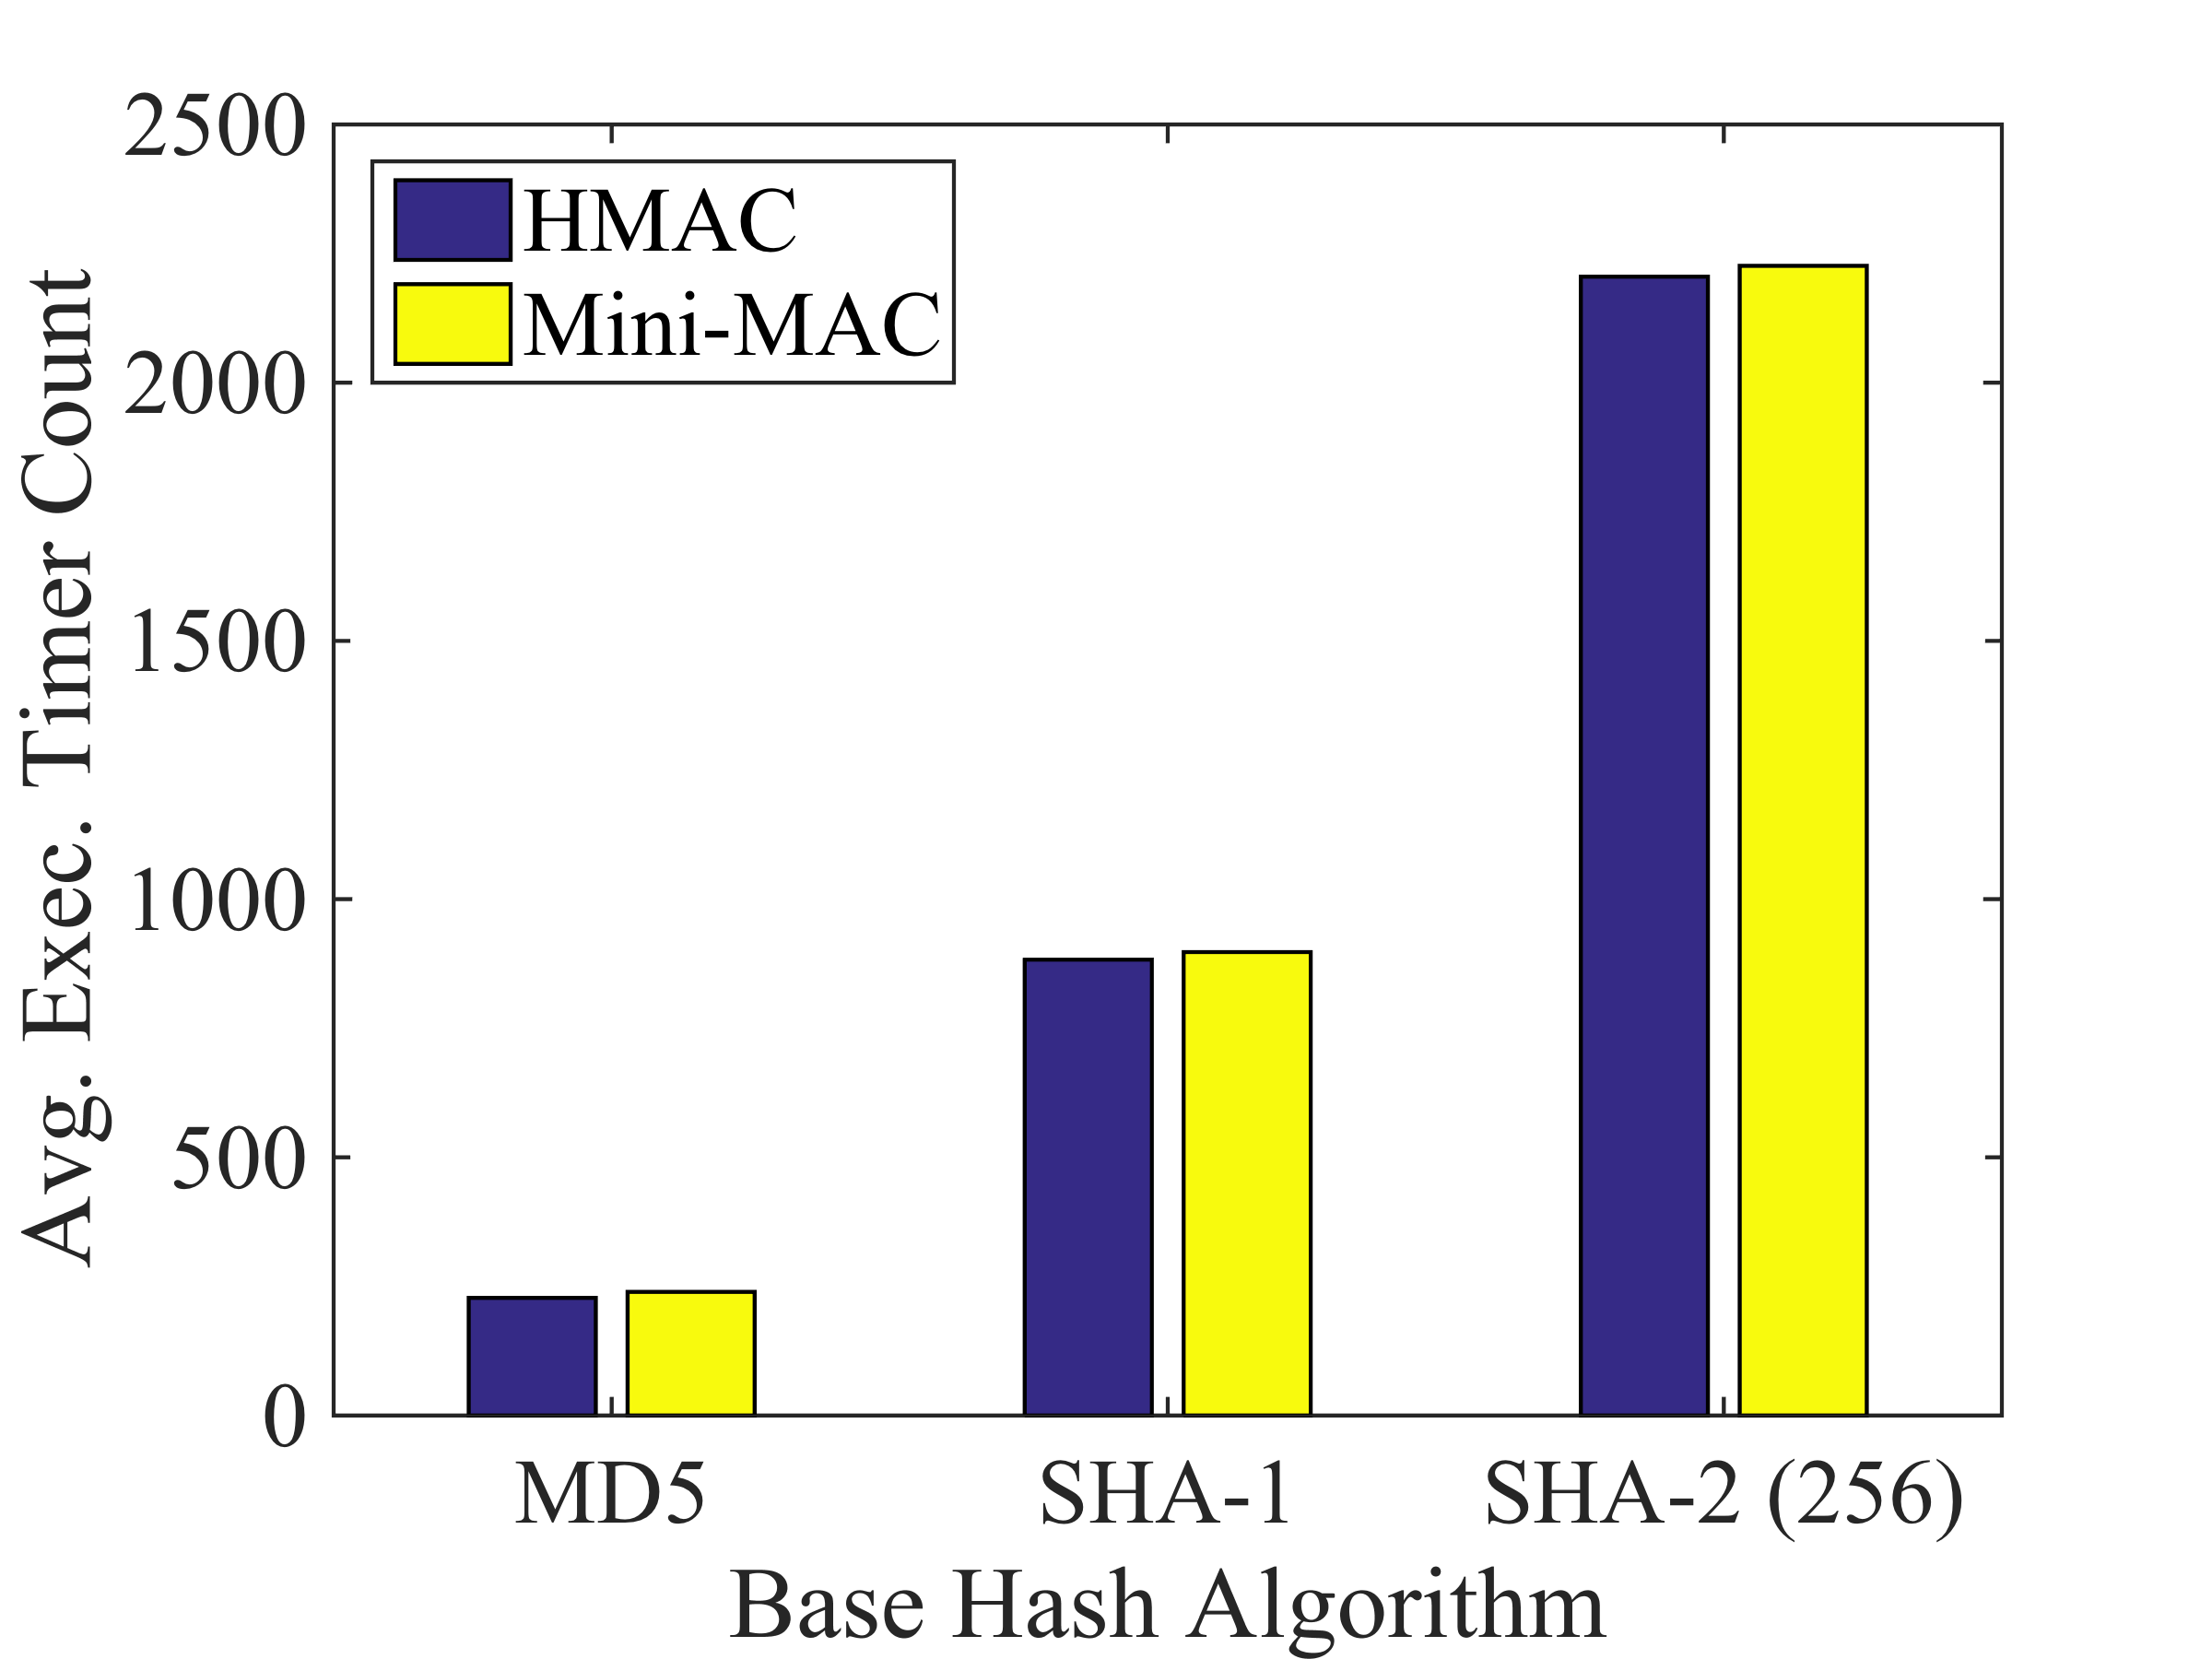
\includegraphics[width=\columnwidth]{figures/exec_cycles.png}
		\caption{Execution Time Comparison of Mini-MAC Construction}
	\end{figure}
	
	\begin{figure}
		\centering
		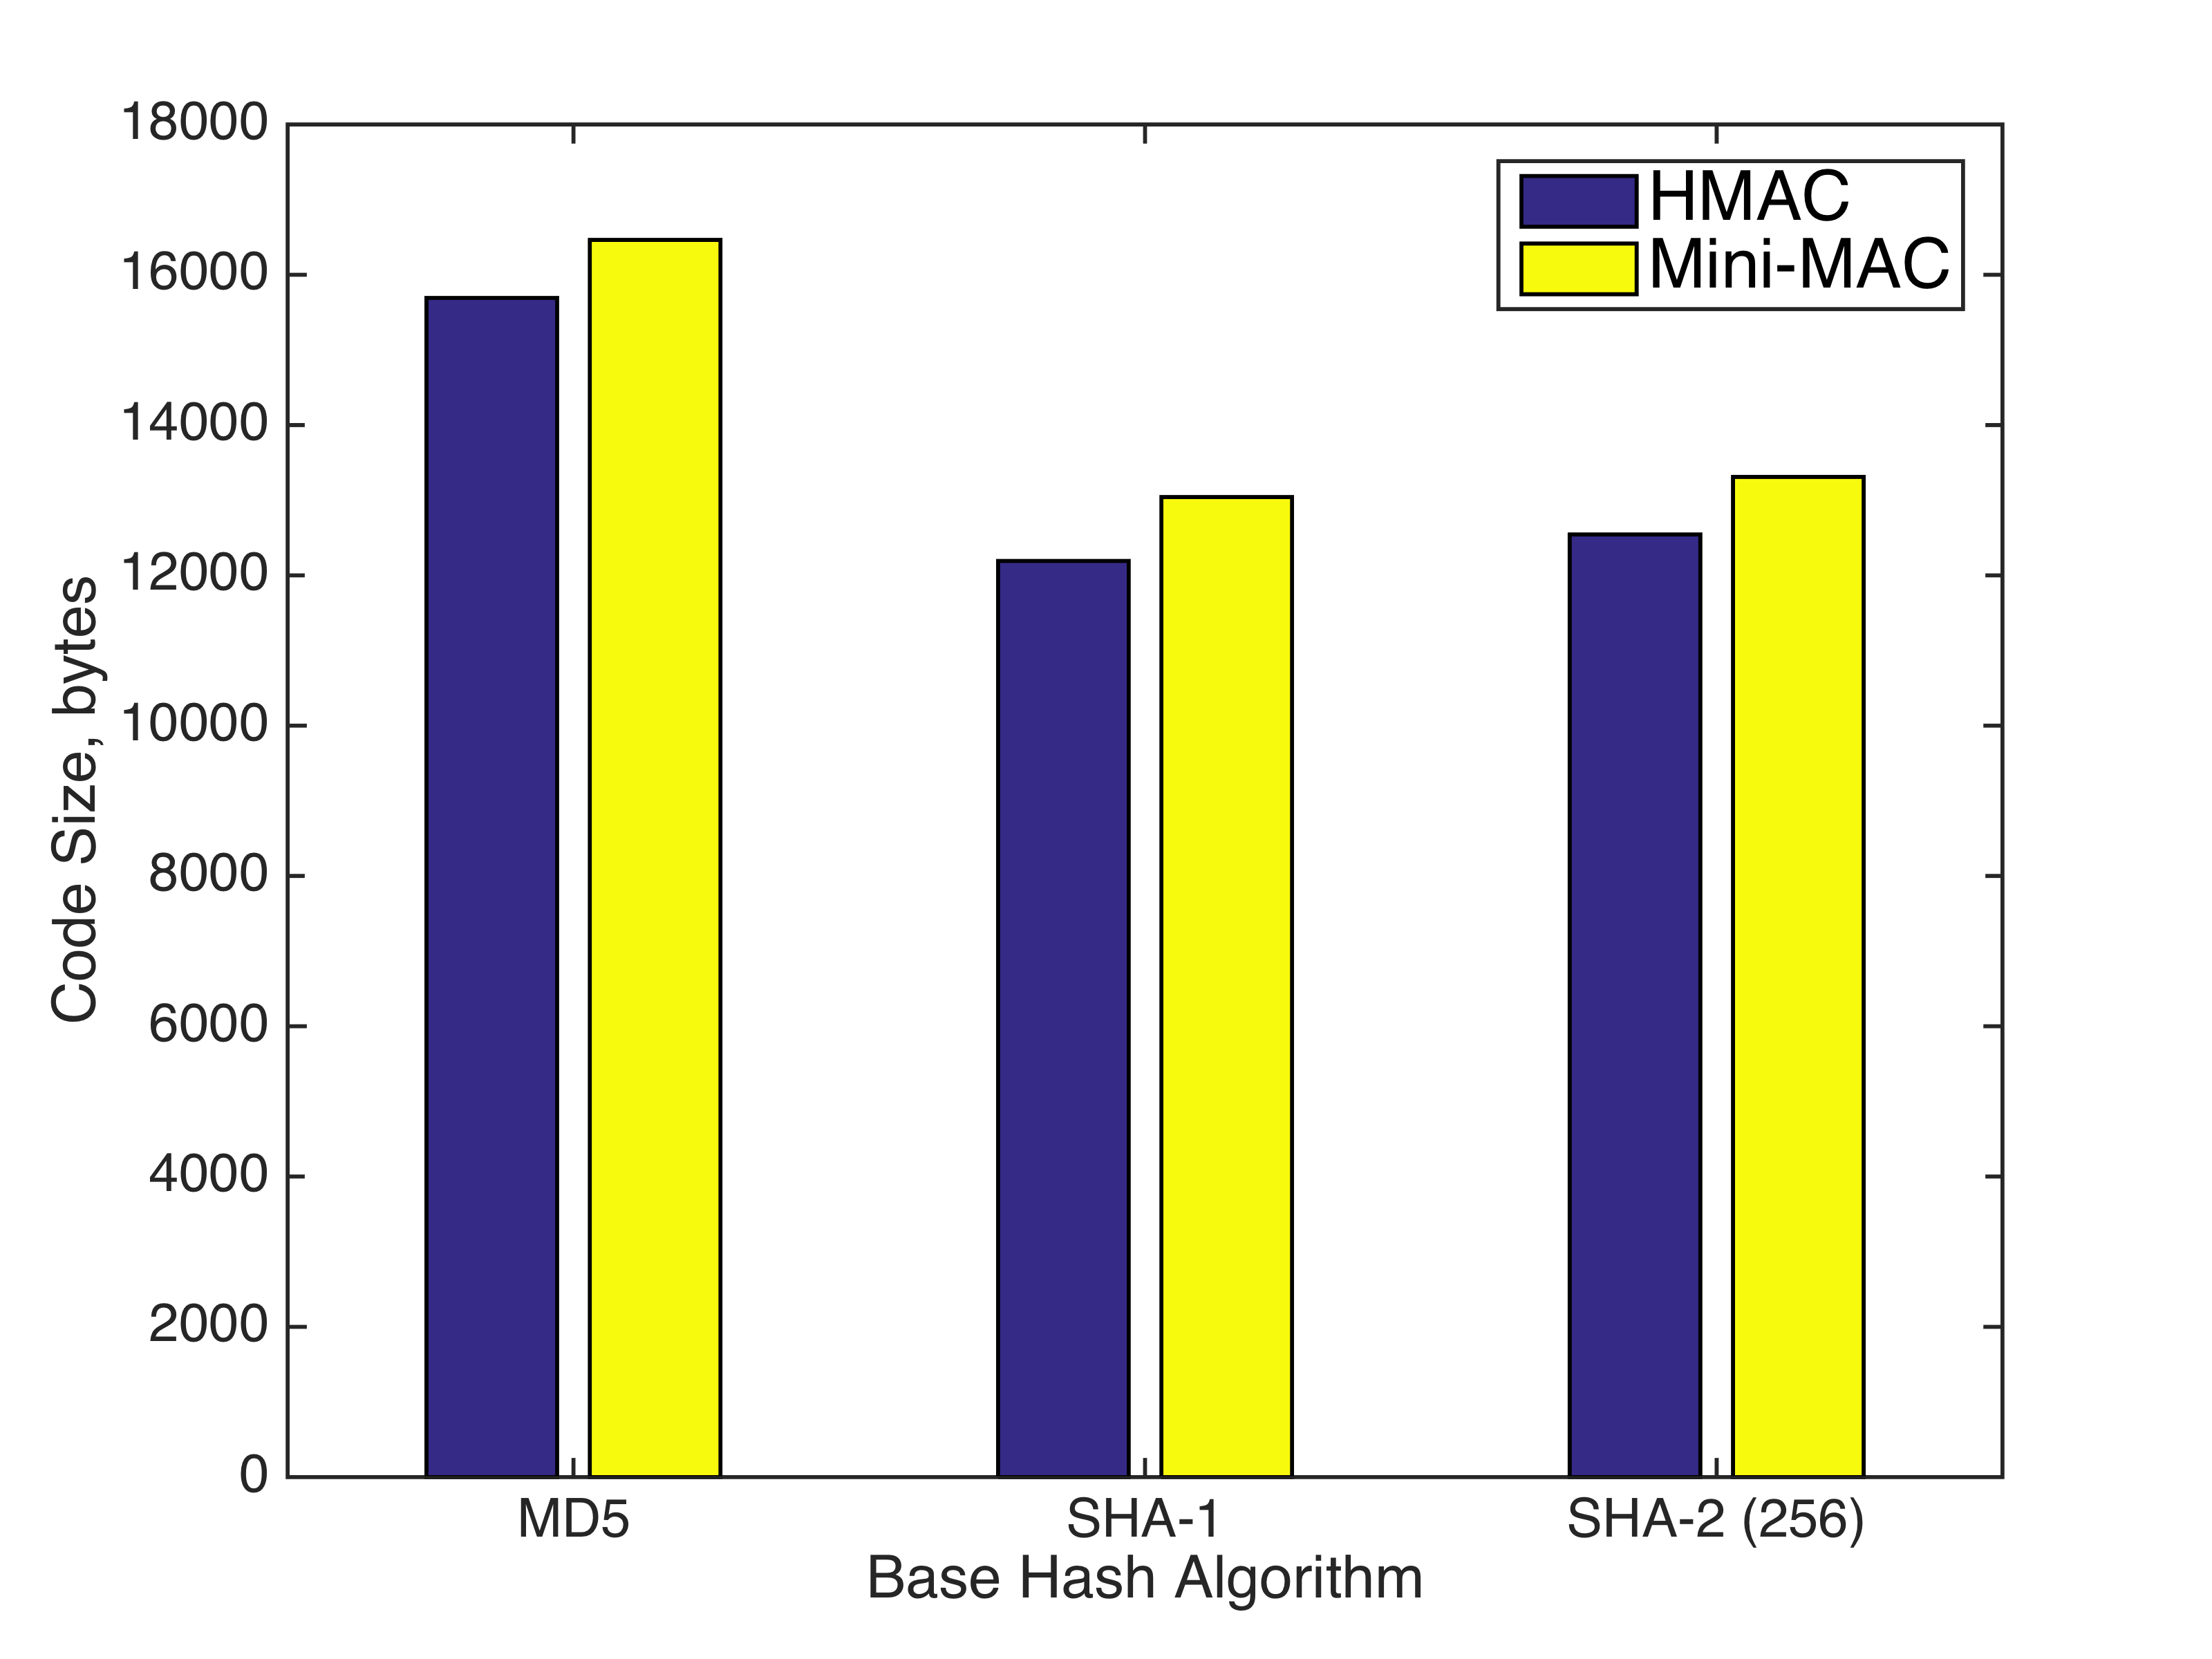
\includegraphics[width=\columnwidth]{figures/code_size.png}
		\caption{Code Size Comparison of Mini-MAC Code}
	\end{figure}
	
	\begin{figure}
		\centering
		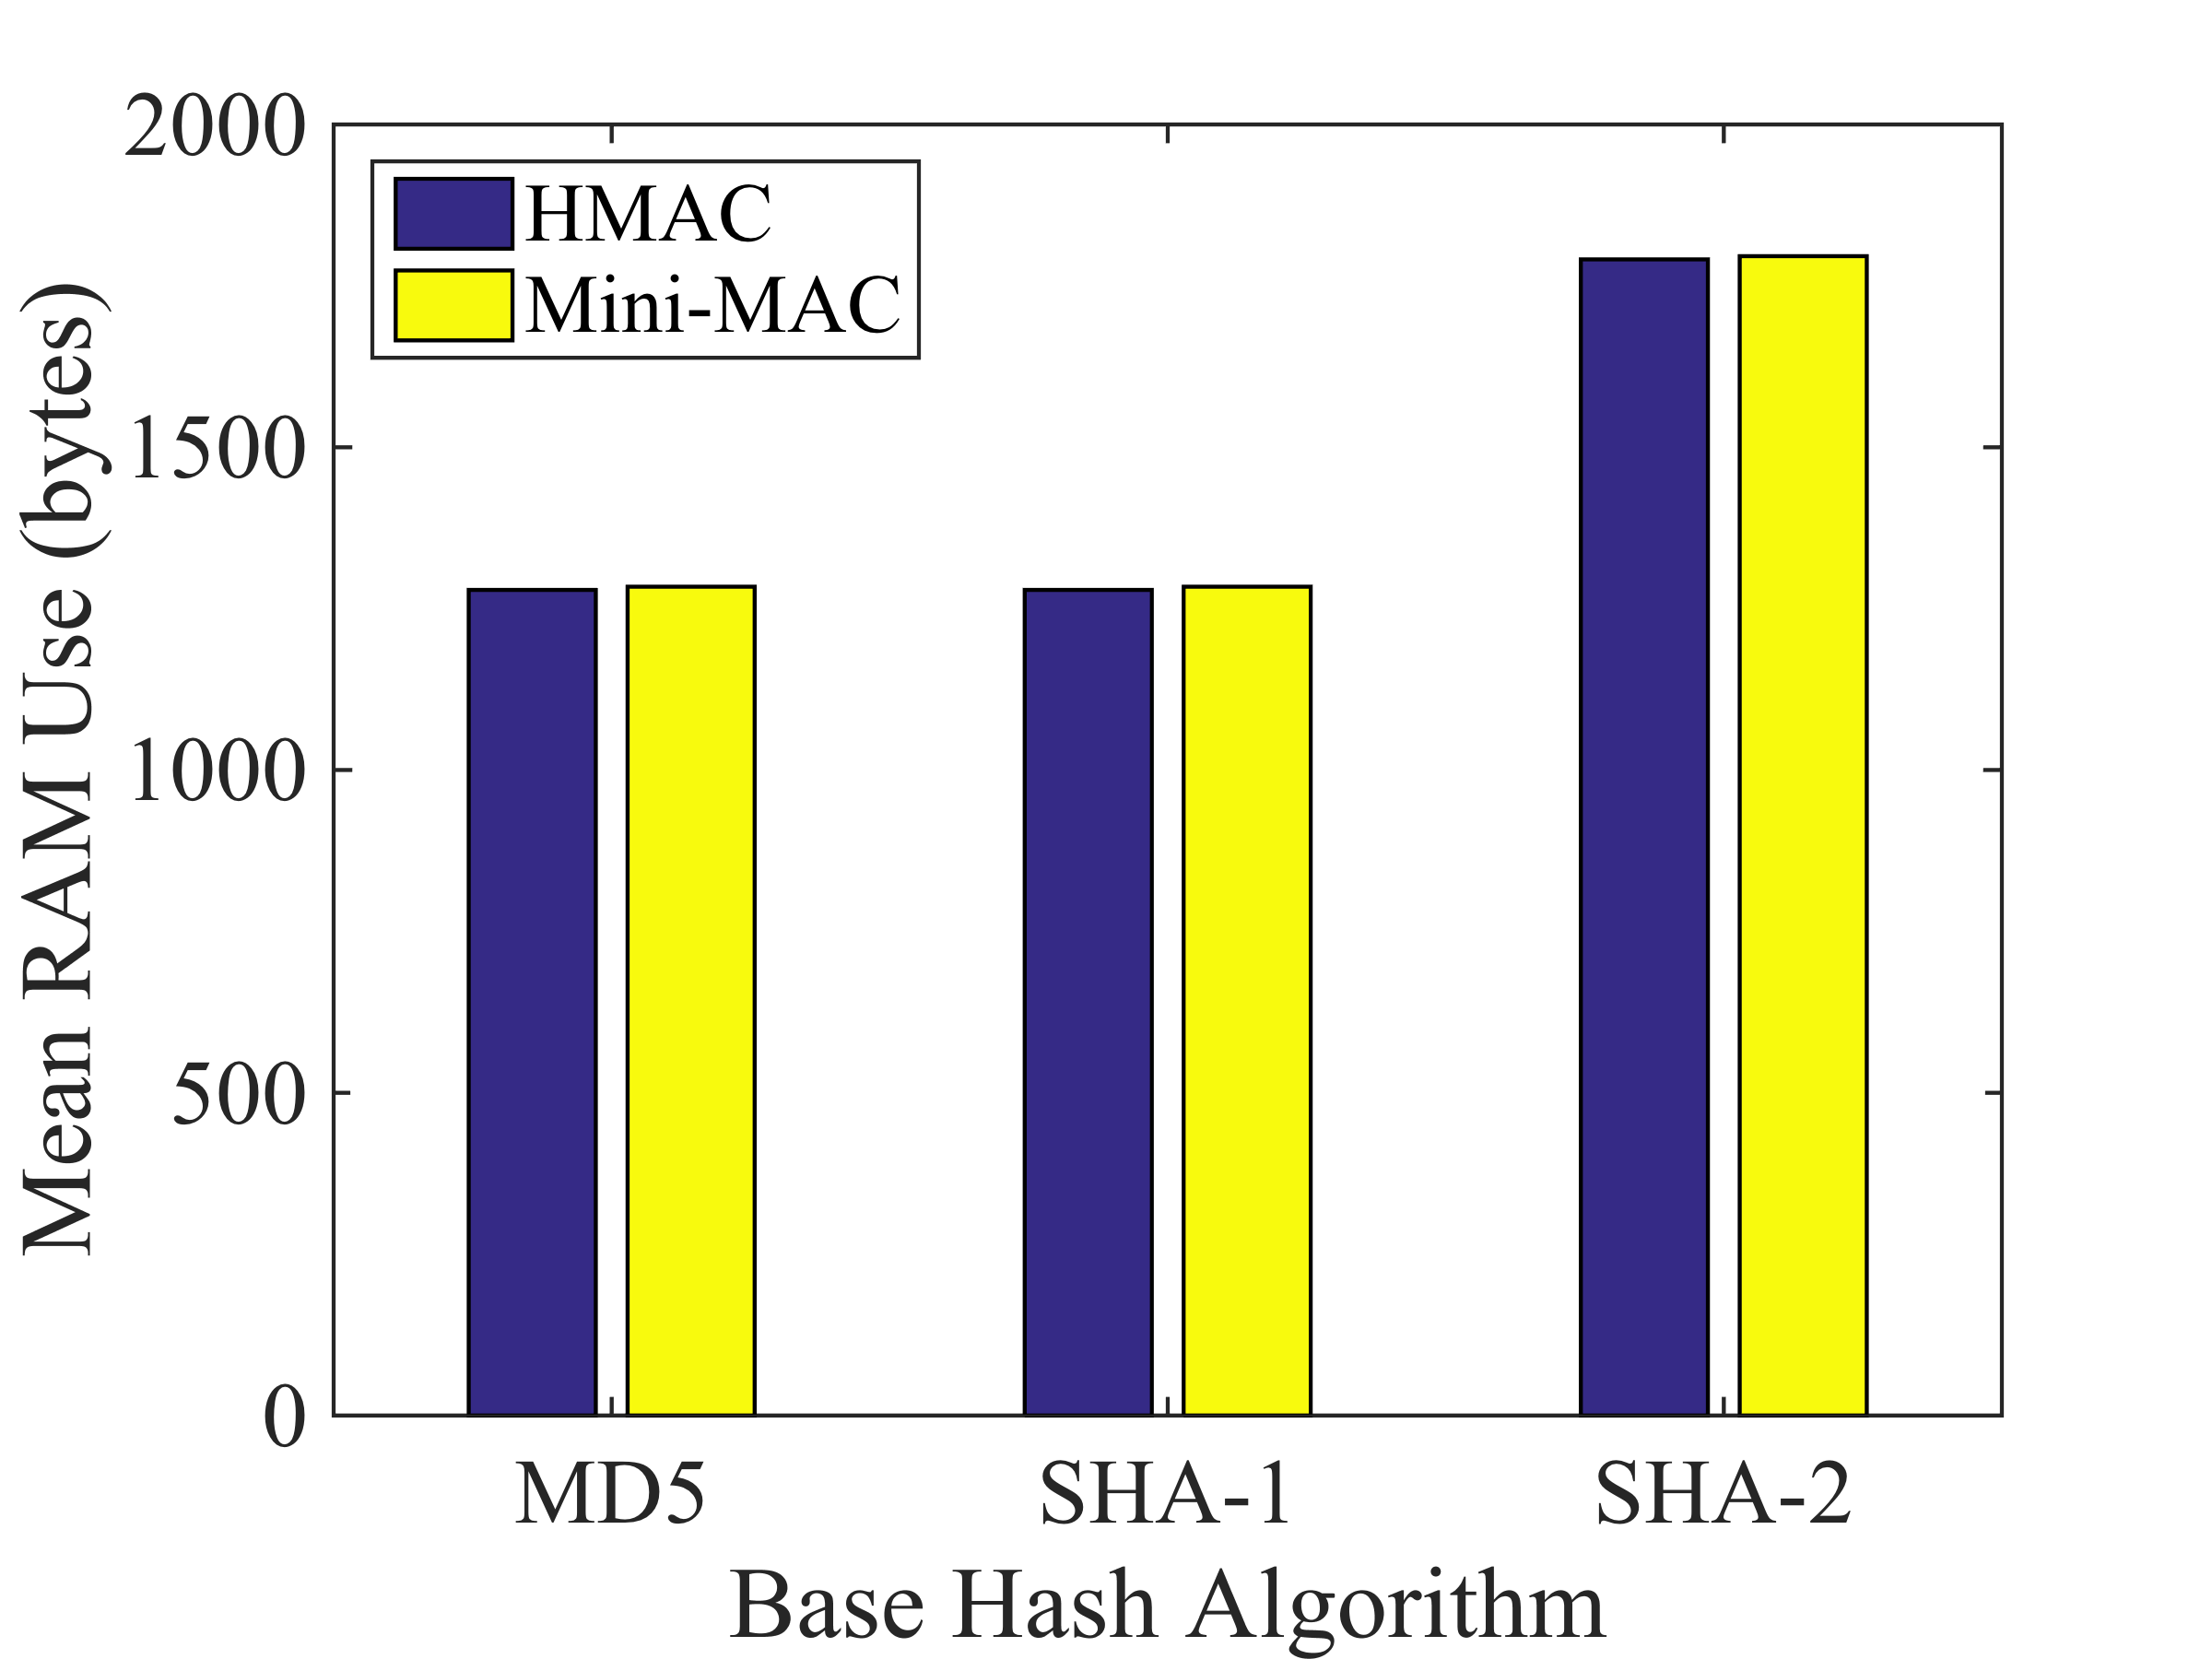
\includegraphics[width=\columnwidth]{figures/ram_usage.png}
		\caption{RAM Usage Comparison of Mini-MAC Code}
	\end{figure}
	